\documentclass[a4paper, 11pt]{article}
\usepackage[utf8]{inputenc}
\usepackage[T1]{fontenc}
\usepackage[margin=1.5cm]{geometry}
\usepackage{graphicx}

\title{Praca inżynierska "Optymalizacja sieci neuronowej za pomocą algorytmów ewolucyjnych"}
\author{Szymon Wasążnik\\325522}
% \date{}

\begin{document}
\maketitle
\section{Cel}
Celem pracy jest opracowanie biblioteki w języku Python,
która umożliwi automatyczne optymalizowanie sieci neuronowej
pod względem architektury sieci na podstawie danych treningowych i walidacyjnych.
Optymalizowanie będzie odbywać się dzięki algorytmowi genetycznemu.

\section{Opis problematyki}
Dobór architektury sieci neuronowej i parametrów uczenia jest procesem,
wymagającym doświadczenia oraz licznych eksperymentów.
W praktyce trzeba testować wiele konfiguracji warstw,
liczby neuronów, funkcji aktywacji czy parametrów uczenia.
Do tego najlepiej testować daną konfigurację kilka razy,
ponieważ są losowane startowe wagi,
które mogą wpływać znacząco na końcowy wygląd sieci po uczeniu.

\noindent\\
Algorytmy genetyczne, pozwalają efektywnie przeszukiwać przestrzeń możliwych modeli
dzieki budowaniu ich na podstawie "genów".
Dzięki tej charakterystyce powinien dobrze sprawdzić się w dobieraniu odpowiedniej architektury i parametrów.

\noindent\\
Celem pracy jest zbudowanie biblioteki,
która automatyzuje proces dobierania przez wspomniany algorytm genetyczny.

\section{Zakres}
Program powininen optymalizować architekturę sieci neuronowej wraz
z jej parametrami uczenia dla danych podanych przez użytkownika.
Dane będą przyjmowane w postaci tabel pakietu \texttt{numpy}.

\noindent
Przez architekturę sieci, w niniejszym dokumencie, rozumie się liczbę warstw,
liczbę neuronów w każdej z warstw oraz funkcje aktywacji dla każdej z warstw.
A przez parametry uczenia rozumie się rodzaj optymalizatora,
wskaźnik uczenia się, funkcję straty, oraz liczbę epok.

\noindent
Optymalizacja powinna się odbywać dla konkretnych danych dostarczonych przez użytkownika,
za pomocą algorytmu genetycznego.
Implementacja algorytmu genetycznego będzie obejmowała:
osobników, selekcję, krzyżowanie i mutację.

\noindent
Każdy osobnik będzie przechowywał jednoznaczny kod genetyczny, to znaczy,
że dany kod genetyczny za każdym razem doprowadzi do takiej samej architektury
wraz z takimi samymi parametrami uczenia.

\noindent
Zostaną przeprowadzone eksperymenty, gdzie będzie spradzane
czy automatycznie dobrane sieci są lepszej lub takiej samej jakości
jak te dobrane manualnie.

\noindent
Zostaną określone domyślne parametry dla algorytmu genetycznego,
które będą możliwie najkorzystniejsze dla optymalizacji architektur sieci neuronowych.

\section{Wstęp teoretyczny}
\subsection{Sieć neuronowa}
Sieć neuronowa to model matematyczny inspirowany działaniem mózgu.
Składa się z sztucznych neuronów (dalej nazywanych neuronami)
oraz synapsów (w terminologi angielskiej występują one pod nazwą \textit{edges}).

\noindent
Obecnie sieci neuronowe są mocno rozwijanym działem informatyki.
Z tego powodu powstało wiele typów sieci,
które można uogólnić do kategorii jednokierunkowa sieć neuronowa
(ang. \textit{feedforward neural networks})
oraz rekurencyjna sieć neuronowa (ang. \textit{recurrent neural networks}).
W angielskiej literaturze można spotkać jeszcze następujące typy sieci:
recursive neural network, feedback neural network.
W niniejszym dokumencie sieci neuronowe odnoszą się
do jednokierunkowej sieci neuronowej (FNN),
a dokładniej do jej szczególnego przypadku nazwanego
wielowarstwowym perceptronem (ang. \textit{multilayer perceptron}).
Jego cechą charakterystyczną jest brak synapsów między warstwami,
które nie są "obok siebie".
Oznacza to, że obie poniższe sieci są jednokierunkowe,
ale tylko ta po prawej jest wielowarstwowym perceptronem (MLP):

\noindent
\begin{center}
  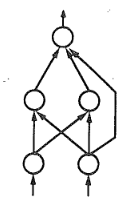
\includegraphics[trim={0 0 0 0}, width=4cm, clip]{fnn.png}
  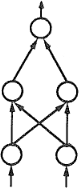
\includegraphics[trim={0 0 0 0}, width=3.25cm, clip]{fnn_mlp.png}
\end{center}

\noindent
W MLP można wyróżnić trzy warstwy: wejściową, ukrytą i wyjściową.
Ponieważ wejściowa warstwa musi być wielkości danych wejściowych,
a warstwa wyjściowa - wyjściowych,
to algorytm musi zajmować się tylko warstwą ukrytą.

\subsection{Architektura sieci neuronowej}
\subsection{Podejście genetyczne do rozwijania architektury}
\end{document}
